%
% main.tex -- Paper zum Thema <particles>
%
% (c) 2020 Autor, OST Ostschweizer Fachhochschule
%
% !TEX root = ../../buch.tex
% !TEX encoding = UTF-8
%
\newcommand{\mytodo}[1]{\textbf{\textcolor{red}{TODO: #1}}}
\newcommand{\mynote}[1]{\textbf{\textcolor{orange}{NOTE: #1}}}
\chapter{Turning Waves into Particles\label{chapter:particles}}
\kopflinks{Turning Waves into Particles}
\begin{refsection}
\chapterauthor{Flurin Brechbühler und Laurin Heitzer}

Wellen treten überall auf, egal ob in Wasser, als Schallwelle, Licht oder in der Elektrotechnik.
Bei den Medien, in denen sich diese Wellen ausbreiten, geht man oft davon aus, dass sie sich linear verhalten.
Viel spannender wird es aber, wenn sich Nichtlinearitäten einschleichen, welche einige interessante Nebeneffekte mit sich bringen.
Solche Nebeneffekte wurden im Video \emph{Turning Waves into Particles}~\cite{particles:huygens-optics} von Huygens Optics (YouTube) gezeigt.
Das Ziel im Video ist, Energie mithilfe der Nichtlinearität des Mediums räumlich zu fangen.

In der folgenden Arbeit wird dieses Phänomen nochmals mathematisch aufgearbeitet. % TODO: Satz passt noch nicht
Es soll der theoretische Hintergrund zu linearen und nichtlinearen Medien erklärt und anhand numerischer Simulation deren Auswirkungen auf die Wellenausbreitung veranschaulicht werden.

%
% teil1.tex -- Beispiel-File für das Paper
%
% (c) 2020 Prof Dr Andreas Müller, Hochschule Rapperswil
%
% !TEX root = ../../buch.tex
% !TEX encoding = UTF-8
%
\section{Lineares Medium\label{particles:section:linear}}
\kopfrechts{Lineares Medium}
% TODO: Quellenangaben
% [ ]: https://en.wikipedia.org/wiki/Linearity
% [ ]: Lineare Algebra: Eine anwendungsorientierte Einführung, Seite: 27, ISBN: 978-3-662-67865-7, Published: 01 September 2023, DOI: https://doi.org/10.1007/978-3-662-67866-4

\subsection{Was ist Linearität?}
Für den einfachsten und üblichsten Fall, nimmt man oft ein \emph{lineares Medium} an.
Solch ein Medium nennt man \emph{linear}, wenn dessen Definition sowohl \emph{additiv}
\[
    f(x_{1} + y_{1}, \ldots, x_{n} + y_{n}) 
    = 
    f(x_{1}, \ldots, x_{n}) 
    + 
    f(y_{1}, \ldots, y_{n}),
\]
als auch \emph{homogen}
\[
    f(\lambda x_{1}, \ldots, \lambda x_{n}) 
    = 
    \lambda f(x_{1}, \ldots, x_{n})
\]
ist.
Hierbei ist angemerkt, dass $x_{k}$, $y_{k}$ und $\lambda$ nicht rein reell sein müssen, 
sondern einem beliebigen Vektorraum angehören können, 
was für den zweidimensionalen Fall wichtig ist.

In der Wellentheorie bedeutet dies, 
dass die Materialeigenschaften---beispielsweise die Elastizität---nicht von der Amplitude der Welle abhängen.
Diese Elastizität eines Mediums lässt sich durch das \emph{hookesche Gesetz}
\[
    \Delta l
    = 
    \frac{F}{D}
    \quad
    \left(D = \text{const.} 
    \Rightarrow 
    \frac{\partial D}{\partial F} 
    \overset{!}{=} 
    0 
    \quad 
    \forall F \right)
    \label{particles:eq:hookesches-gesetz},
\]
welches bereits in abschnitt \mytodo{Verweis Elastizitätstheorie} verwendet wurde, beschreiben.
Dabei beschreibt $\Delta l$ die Distanzänderung zweier Punkte,
$F$ die dazwischen wirkende Kraft und $D$ einen Proportionalitätsfaktor.
Mittels Substitution kann man nun darauf schliessen, 
dass es sich hierbei tatsächlich um eine lineare Funktion handeln muss.


\subsection{Superpositionsprinzip}\label{particles:section:lin-medium:superposition}
Das Superpositionsprinzip fasst die Bedingungen zur Linearität nochmal etwas schöner in eine Formel zusammen, 
nämlich
\[
    T(\lambda x + \mu y)
    = 
    \lambda T(x) 
    + 
    \mu T(y).
\]
Blickt man wieder auf die Wellentheorie, so bedeutet dies, 
dass sich Wellen in linearen Medien überlagern, 
sich aber nicht gegenseitig beeinflussen.
Dies kann man schön anhand zweier sich kreuzende Laserstrahlen im Vakuum veranschaulichen, 
wie sie in Abbildung \mytodo{Abbildung zweier Laserstrahlen, die sich kreuzen, lokal interferieren, jedoch den weiteren Verlauf nicht verändern.} gezeigt werden.
Lokal interferieren diese Laserstrahlen zwar, stören jedoch nicht ihren weiteren Verlauf. 

\mytodo{Irgendwo sollte man noch ein Beispiel mit $E$- oder $B$-Feld einbringen}


\subsection{Schwinger-Limit}\label{particles:section:lin-medium:schwinger}
Bei extrem hohen Feldstärken tritt ein Phänomen auf, wobei das Vakuum selbst nichtlinear wird.
Dieser Übergang zur Nichtlinearität des Vakuums nennt man das \emph{Schwinger-Limit}\mytodo{Quellenangabe}, benannt nach Julian Schwinger, welcher 1951 dieses Phänomen erstmals theoretisierte.
Da es sich hierbei um elektrische und magnetische Feldstärken im Bereich von $10^{18}\,\frac{\text{V}}{\text{m}}$ und $10^9\,\text{T}$ handelt, konnte dieses Limit bisher noch nicht konkret nachgewiesen oder gemessen werden.
Es ist entsprechend noch immer Bestandteil aktueller Forschungen. \mytodo{Quelle hierfür angeben}

Beschränkt man sich jedoch nicht nur auf das Vakuum, so findet man Medien, welche bereits bei deutlich kleineren Feldstärken nichtlineare Eigenschaften aufweisen.
Ein Beispiel von solchen nichtlinearen Werkstoffen sind, wie~\ref{particles:frequenzverdopplung} demonstriert, Kristalle zur Frequenzverdoppelung.
Diese werden zum Beispiel in grünen Laserpointern eingesetzt, was die Verwendung von preiswerteren Infrarot-Laserdioden anstelle der teureren grünen Ausführung erlaubt.

% TODO Teil 1:
% - Was ist Linearität?
% - Superposition
% - Grenze der Linearität: Schwinger-Limit
%
% einleitung.tex -- Beispiel-File für die Einleitung
%
% (c) 2020 Prof Dr Andreas Müller, Hochschule Rapperswil
%
% !TEX root = ../../buch.tex
% !TEX encoding = UTF-8
%
\section{Simulation\label{particles:section:simulation}}
\kopfrechts{Simulation}

Für die konventionelle Wellengleichung~\eqref{particles:eq:wellengleichung} 
können Lösungen besonders für einfache Fälle auch analytisch gefunden werden.
Sobald jedoch das Medium nichtlinear und 
der Proportionalitätsfaktor $c$ nicht mehr unabhängig von der Deformation $u$ ist, 
wird eine analytische Lösung beinahe unmöglich.
Entsprechend wurde in der Hinsicht darauf, 
dass schliesslich auch nichtlineare Medien simuliert werden können, 
ein numerischer Ansatz gewählt.

So wurde für die Simulationen eine von \emph{Dr. Jeroen Vleggaar} angepasste Version des Open-Source Wellensimulators WaveSimulator2D~\cite{particles:repo-wavesim2d} verwendet.
Dieser simuliert eine zweidimensionale Szene, indem er die Wellengleichung für einen diskreten Zeitschritt simuliert und das resultierende Feld anzeigt.
Die Szene wird dabei ebenfalls örtlich diskretisiert, indem sie in Pixel aufgeteilt wird.

\subsection{Wellengleichung\label{particles:section:simulation:wellengleichung}}
Die Diskretisierung der Raumdimensionen erlaubt die Berechnung von $\nabla^2 u$ als Faltung des Felds $u$ mit einem Laplace kernel.
WaveSimulator2D verwendet dazu den Kernel
\[
    \mathbf{D}^2_{xy} = 
    \begin{pmatrix}
        0.066 &  0.184 & 0.066\\
        0.184 & -1.000 & 0.184\\
        0.066 &  0.184 & 0.066\\
    \end{pmatrix},
\]
was zu der angepassten Wellengleichung 
\[
    \frac{\d^2 u}{\d t^2} = c^2 \cdot (\mathbf{D}^2_{xy} * u)
\]
führt.

Für die Ableitung im Zeitbereich wird der zentrale Differenzquotient
\[
    \frac{\d^2 u(t)}{\d t^2} \approx \frac{u(t-T) - 2u(t) + u(t+T)}{T^2}
\]
eingesetzt.
$T$ ist dabei der diskrete Zeitschritt der Simulation.

Die angepasste Wellengleichung 
\[
    \frac{u(t-T) - 2 u(t) + u(t+T)}{T^2} = c^2 \cdot (\mathbf{D}^2_{xy} * u)
\]
kann nun nach $u(t+T)$, also nach dem Wert von $u$ einen Zeitschritt in der Zukunft, umgestellt werden, was in
\[
    \underbrace{%
        u(t+T) = 2 u(t) - u(t+T) + T^2      % Equation part 1
        \vphantom{\mathbf{D}^2_{xy}}        % Adjust height
    }_{%
        \textstyle
        \frac{\d^2 u(t)}{\d t^2}            % Description
    } 
    \cdot 
    \underbrace{%
        c^2 \cdot (\mathbf{D}^2_{xy} * u)   % Equation part 2
    }_{%
        \textstyle
        \nabla^2 u                          % Description
        \vphantom{\frac{\d^2 u(t)}{\d t^2}} % Adjust height
    }
\]
resultiert.
Diese Gleichung kann verwendet werden, um ungedämpfte Wellen in linearen Medien zu simulieren.

\subsection{Dämpfung}
Damit der später erwähnte Farbkanal zur Dämpfung des Mediums realisiert werden kann, 
wird die Wellengleichung durch einen Dämpfungsterm erweitert.
Die angepasste Wellengleichung 
\[
    \frac{\d^2 u}{\d t^2} + d \frac{\d u}{\d t}= c^2 \cdot \nabla^2 u
\]
mit der Dämpfung $d$ als Skalarfeld kann entlang dem selben Weg wie in Abschnitt~\ref{particles:section:simulation:wellengleichung} dargestellt nach $u(t+T)$ umgeformt werden.
Dabei wird für die Ableitung $\frac{\d u}{\d t}$ der einseitige Differenzquotient
\[
    \frac{\d u}{\d t} \approx \frac{ - u(t-T)}{T}
\]
verwendet.

Die resultierende Wellengleichung lautet
\[
    \underbrace{%
        u(t+T) = 2 u(t) - u(t+T) + T^2      % Equation part 1
        \vphantom{\mathbf{D}^2_{xy}}        % Adjust height
    }_{%
        \textstyle
        \frac{\d^2 u(t)}{\d t^2}            % Description
    } 
    \cdot 
    \underbrace{%
        c^2 \cdot (\mathbf{D}^2_{xy} * u)   % Equation part 2
    }_{%
        \textstyle
        \nabla^2 u                          % Description
        \vphantom{\frac{\d^2 u(t)}{\d t^2}} % Adjust height
    }
     - 
    \underbrace{%
        d \cdot T \cdot (u(t) - u(T-1))
        \vphantom{\mathbf{D}^2_{xy}}        % Adjust height
    }_{%
        \textstyle
        d \cdot \frac{\d u(t)}{\d t}        % Description
    }.
\]

\subsection{Nichtlinearität}
Die Nichtlinearität des Mediums wird durch die Formel
\[
    \text{stress} = a \cdot \text{strain} \cdot e^{b \cdot \text{strain}} % TODO: Tatsächliche Formel
\]
gegeben, wobei das nichtlineare Verhalten durch die Parameter $a$ und $b$ angepasst werden kann.
Einige Beispiele der daraus resultierenden Spannungs-Deformations-Kurven sind in Abbildung~\ref{particles:abb:nonlin} gezeigt. % TODO: Abbildung
\mytodo{Beschreiben, wie der Simulator das einrechnet}

\subsection{Szenendefinition}
Zur Definition des Ausgangszustands des Feldes sowie der Eigenschaften des Mediums nimmt der Simulator ein RGB-Bild entgegen.
Den drei Farbkanälen wird jeweils eine Funktion zugeteilt.
Der rote Kanal bestimmt den Brechungsindex des jeweiligen Pixels, während über den blauen Kanal die Dämpfung bestimmt werden kann.
Über den grünen Kanal können im unveränderten Simulator Quellen dargestellt werden, wobei der Farbwert die Frequenz der Quelle darstellt.
Damit die in der Simulation enthaltene Energie nicht fortlaufend ansteigt, wurde die Funktion des grünen Kanals durch \emph{Dr. Jeroen Vleggaar} angepasst. % TODO: Echter Name von Huygens einfügen
Der grüne Kanal diktiert nun das Spannungsfeld zu Beginn der Simulation. % CHECK: ist es die Spannung oder die Deformation?
% TODO: Beispielszene

\subsection{Performance} % TODO: Evtl. weg lassen...
Die Simulation ist trotz relativ tiefer Auflösung nicht trivial. 
Der WaveSimulator2D zieht Nutzen aus der \texttt{CuPy} Bibliothek um die Faltung des Laplace Kernels mit den aktuellen Feldwerten auf der Grafikkarte laufen zu lassen.
 % TODO: Was passiert bei Nichtlinearitäten
% TODO Teil 2:
% - Definition, Beispiele
% - Schwinger-Limit in der Praxis (?)
% - Selbstfokussierung / Confined Energy
% - Soliton
%
% teil2.tex -- Beispiel-File für teil2 
%
% (c) 2020 Prof Dr Andreas Müller, Hochschule Rapperswil
%
% !TEX root = ../../buch.tex
% !TEX encoding = UTF-8
%
\section{Nichtlineares Medium
\label{particles:section:nichtlinear}}
\kopfrechts{Nichtlineares Medium}
Entgegen des linearen Mediums, in dem der Proportionalitätsfaktor nicht von der wirkenden Kraft abhängig ist, 
wird dies bei einem nichtlinearen Medium nun zum Problem.
Dies bedeutet also, dass sich das hookesche Gesetz von 
\[
    \Delta l
    = 
    \frac{F}{D}
\]
zu
\[
    \Delta l
    = 
    \frac{F}{D(F)}
\]
abändert. 
Wie dieser Proportionalitätsfaktor genau von der Kraft abhängt, ist je nach Medium unterschiedlich.
Ein Beispiel davon wird im Video~\cite{particles:huygens-optics} von Huygens Optics gezeigt, wobei für $D$ die Formel 
\[
    D(F)
    =
    D_0
    \cdot
    (1 + \alpha |F|^n)
\]
eingesetzt wird. Ein Beispiel der daraus resultierenden Graphen ist in \autoref{particles:fig:nichtlin-medium:deform} und \autoref{particles:fig:nichtlin-medium:elast-modul} abgebildet.
\begin{figure}
    \centering
    \subfigure[]{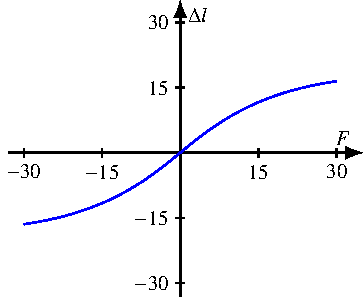
\includegraphics{./papers/particles/figures/out/nichtlineares_medium_deformation.pdf}\label{particles:fig:nichtlin-medium:deform}}\hfill
    \subfigure[]{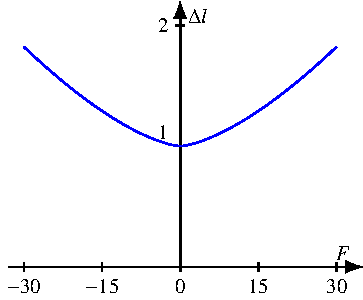
\includegraphics{./papers/particles/figures/out/nichtlineares_medium_elast_modul.pdf}\label{particles:fig:nichtlin-medium:elast-modul}}
    \caption{Deformation~(a) und Elastizitätsmodul~(b) eines nichtlinearen Mediums mit $D_0 = 1$, $\alpha = 0.005$ und $n = 1.5$.}
\end{figure}

Wiederholen wir nun wieder die Simulation aus \autoref{particles:section:lin-medium:superposition}, so fällt zunächst kein Unterschied auf.
\autoref{particles:fig:nichtlin-medium:beams} zeigt einen Vergleich der beiden Resultate.
Damit die Auswirkung der nichtlinearen Effekte erkannt werden können, müssen die Feldstärken scheinbar bedeutend grösser sein.
\begin{figure}
    \centering
    \subfigure[0:20]{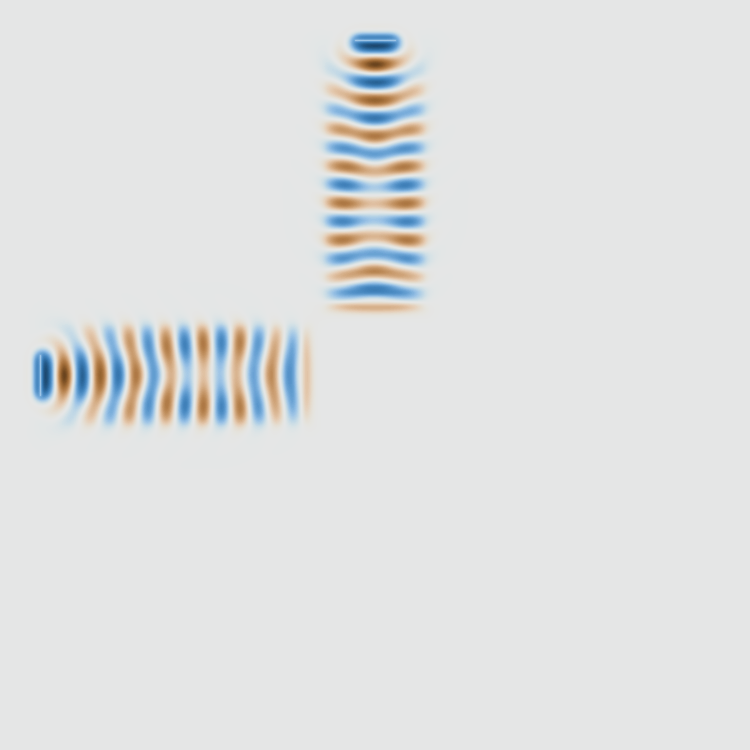
\includegraphics[width=.32\linewidth]{./papers/particles/figures/simulations/beams_nonlin_1_10.png}}\label{particles:fig:nichtlin-medium:beams-1}\hfill
    \subfigure[0:40]{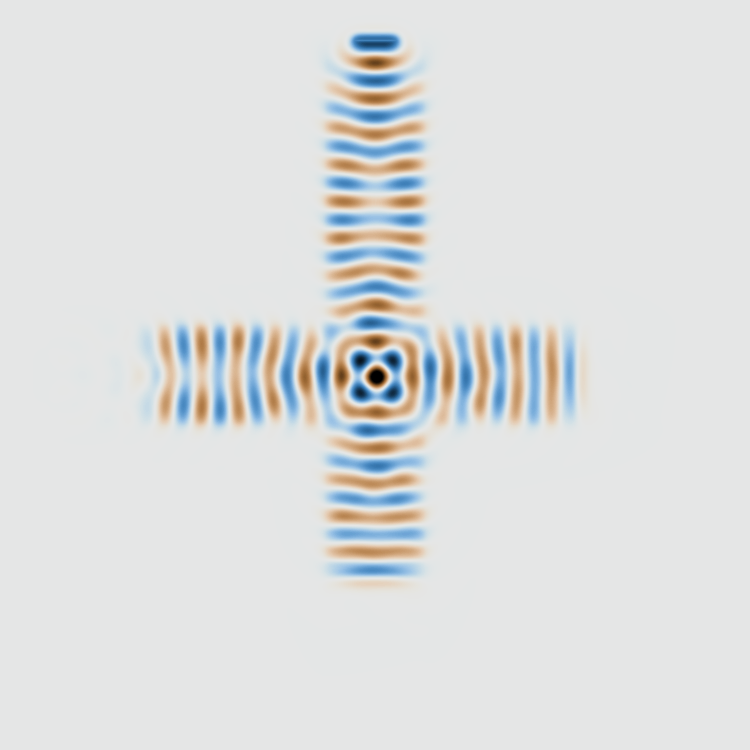
\includegraphics[width=.32\linewidth]{./papers/particles/figures/simulations/beams_nonlin_3_20.png}}\label{particles:fig:nichtlin-medium:beams-2}\hfill
    \subfigure[1:04]{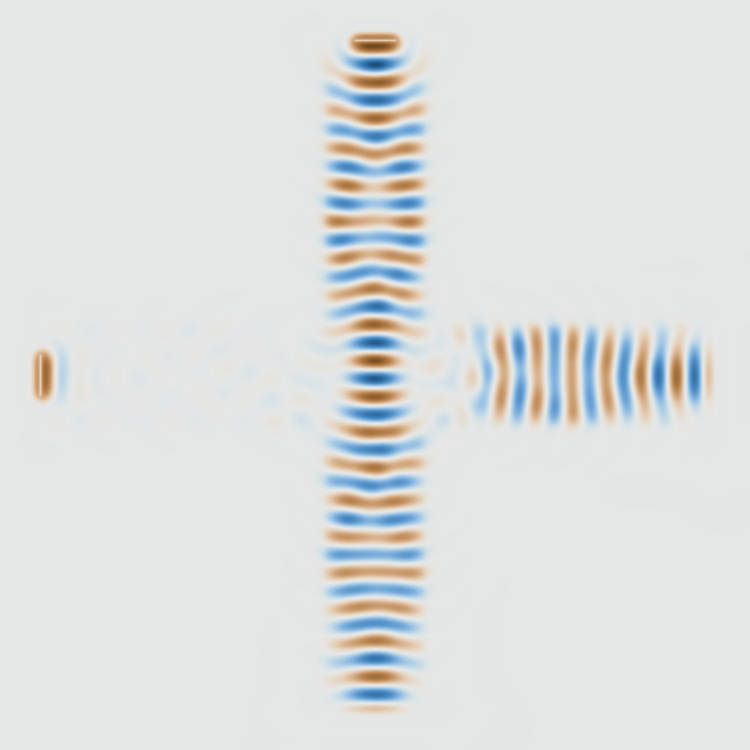
\includegraphics[width=.32\linewidth]{./papers/particles/figures/simulations/beams_nonlin_4_32.png}}\label{particles:fig:nichtlin-medium:beams-3}
    \caption{Strahlen im nichtlinearen Medium zu Beginn~(a), während sie sich kreuzen~(b) und danach~(c) mit den jeweiligen Zeitstempeln.}\label{particles:fig:nichtlin-medium:beams}
\end{figure}


\subsection{Selbstfokussierung -- Confined Energy}
% TODO: Was für Bedingungen müssen erfüllt sein, damit dies geschieht? 
%       Kann man das überhaupt so einfach klassifizieren?
%       Allenfalls Analogie zu Schwingkreisen herstellen?
\begin{figure}
    \begin{center}
        % 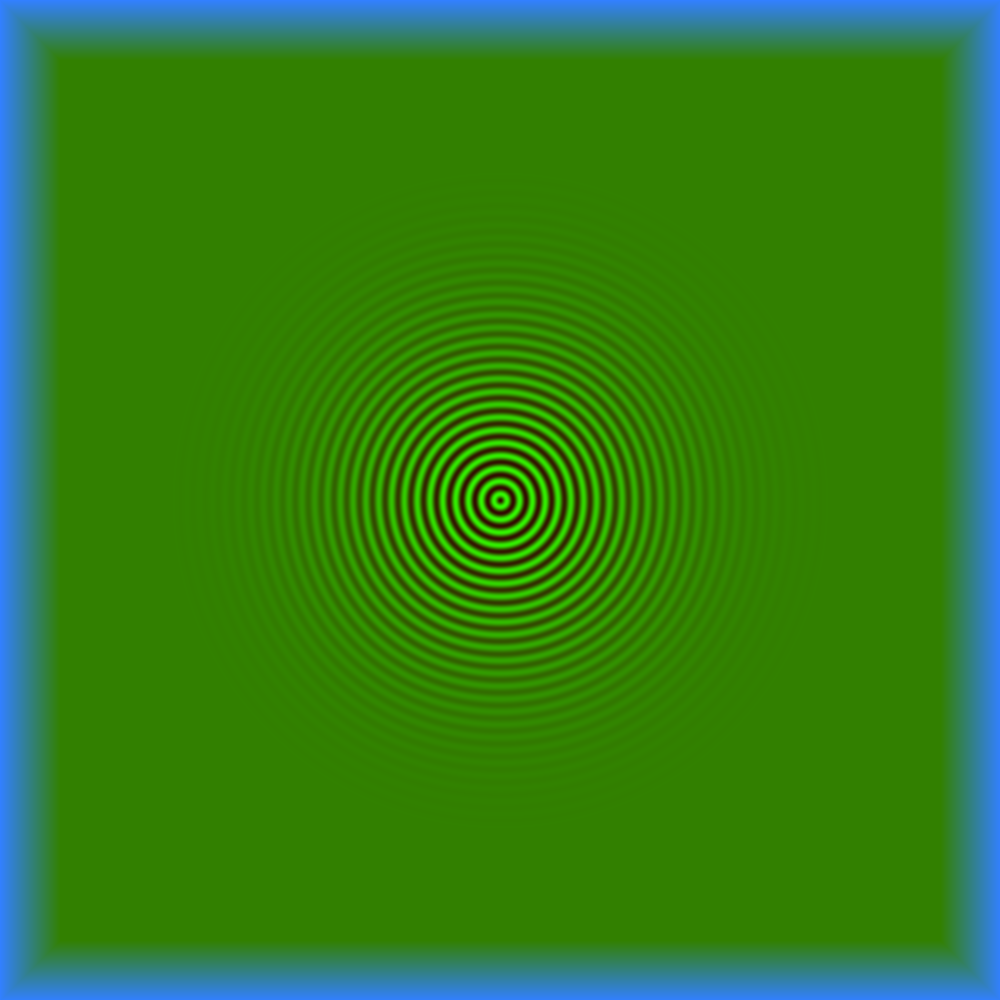
\includegraphics[width=0.5\textwidth]{papers/particles/figures/wavesim/particle_initial_state.png}
        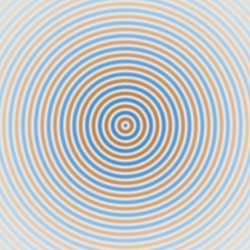
\includegraphics[width=0.5\textwidth]{papers/particles/figures/simulations/particle_frames/frame_00.png}
        \caption{Ausgangszustand zur Zeit 0:00, der zu sehr hohen Feldstärken und schliesslich einer Energieansammlung im Zentrum des Simulationsfelds führt.}\label{particles:fig:partikel:ausgangszustand}
    \end{center}
\end{figure}
\begin{figure}
    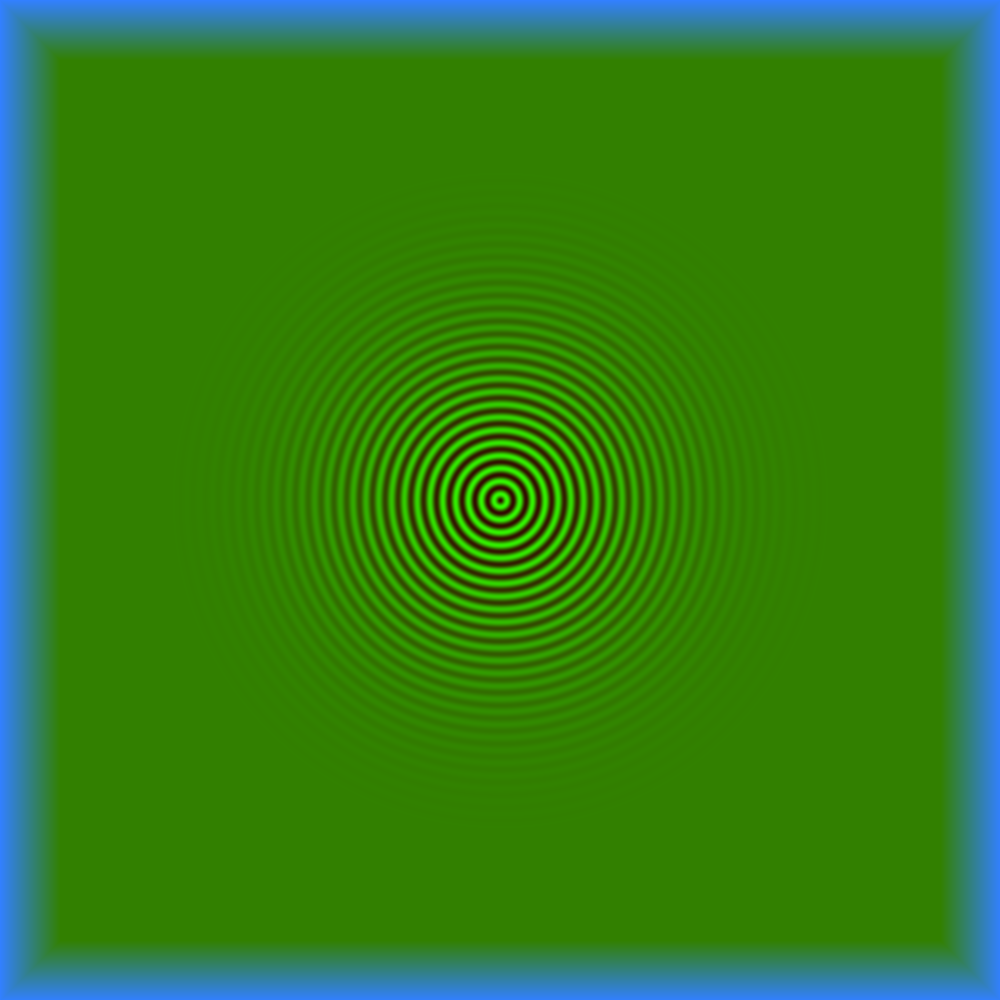
\includegraphics{papers/particles/figures/wavesim/particle_initial_state.png}
    \caption{Feldkonfigurationen mit zunehmend wachsender Energieansammlung im Zentrum der Simulation.\ \mytodo{Bild anpassen}}\label{particles:fig:partikel:wachsen}
\end{figure}
Der in Abbildung~\ref{particles:fig:partikel:ausgangszustand} gezeigte Anfangszustand kann durch das Aufeinandertreffen der Wellen im Zentrum besonders grosse Feldstärken hervorrufen.
Wird die Simulation nun abgespielt, so geschieht etwas Unerwartetes: Die Energie im Feld scheint sich im Zentrum zu sammeln.
Die besondere Region inmitten des Simulationsfelds wächst, 
bis die im Ausgangszustand definierten Wellen entweder gegen den Rand der Simulation verschwinden oder ihre Energie in die Region im Zentrum gesteckt haben.
Dieser Prozess wird in den Abbildungen~\ref{particles:fig:partikel:wachsen-1} und~\ref{particles:fig:partikel:wachsen-2} veranschaulicht.

\begin{figure}
    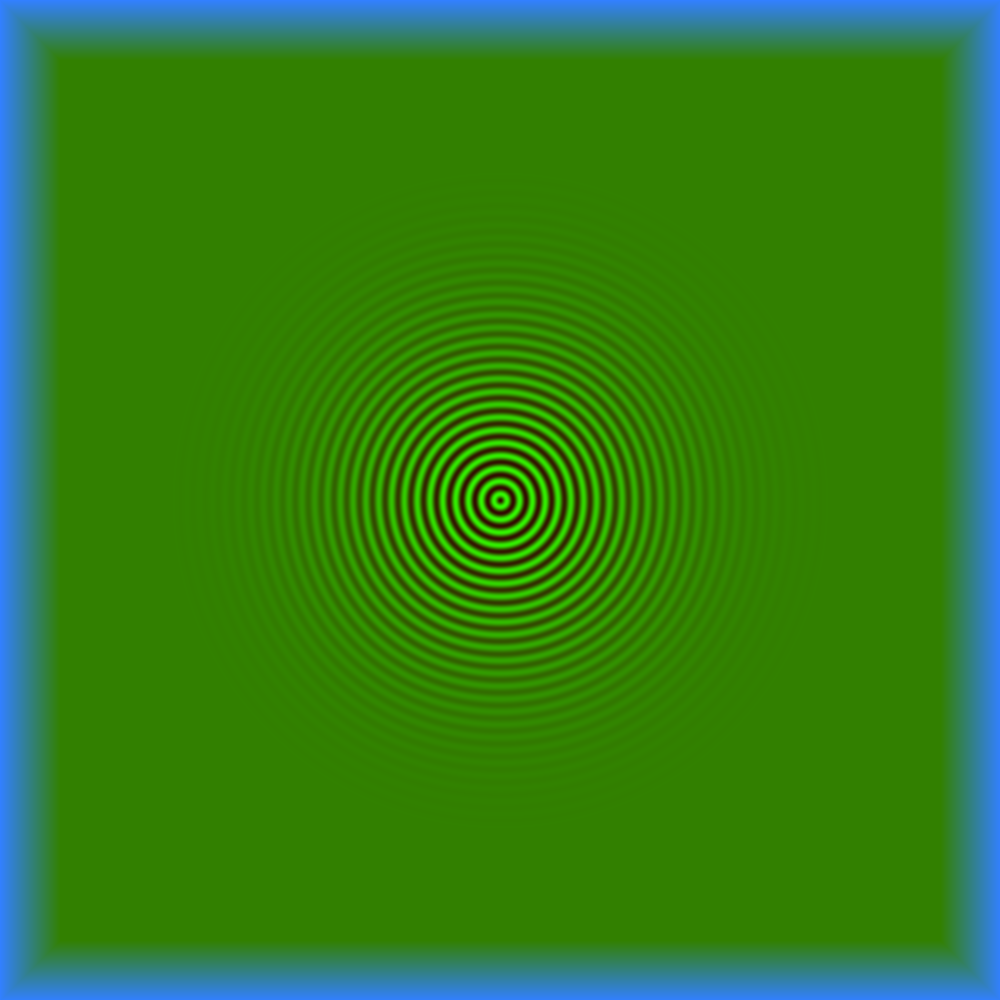
\includegraphics{papers/particles/figures/wavesim/particle_initial_state.png}
    \caption{Symmetrische Feldkonfiguration mit langsahm abnehmender Energiekonsentration.\ \mytodo{Bild anpassen}}\label{particles:fig:partikel:abnehmen:symmetrisch}
\end{figure}
Die nächste Phase zeichnet sich durch Oszillieren der symmetrischen Feldanordnung aus. 
Weiter sind einige schwache Wellen zu erkennen, welche die Region der konzentrierten Energie verlassen.
So schrumpft die gefangene Energie wie auch die Grösse der Feldanordnung fortlaufend.
Einige Bilder sind in Abbildung~\ref{particles:fig:partikel:abnehmen:symmetrisch} gezeigt.

\begin{figure}
    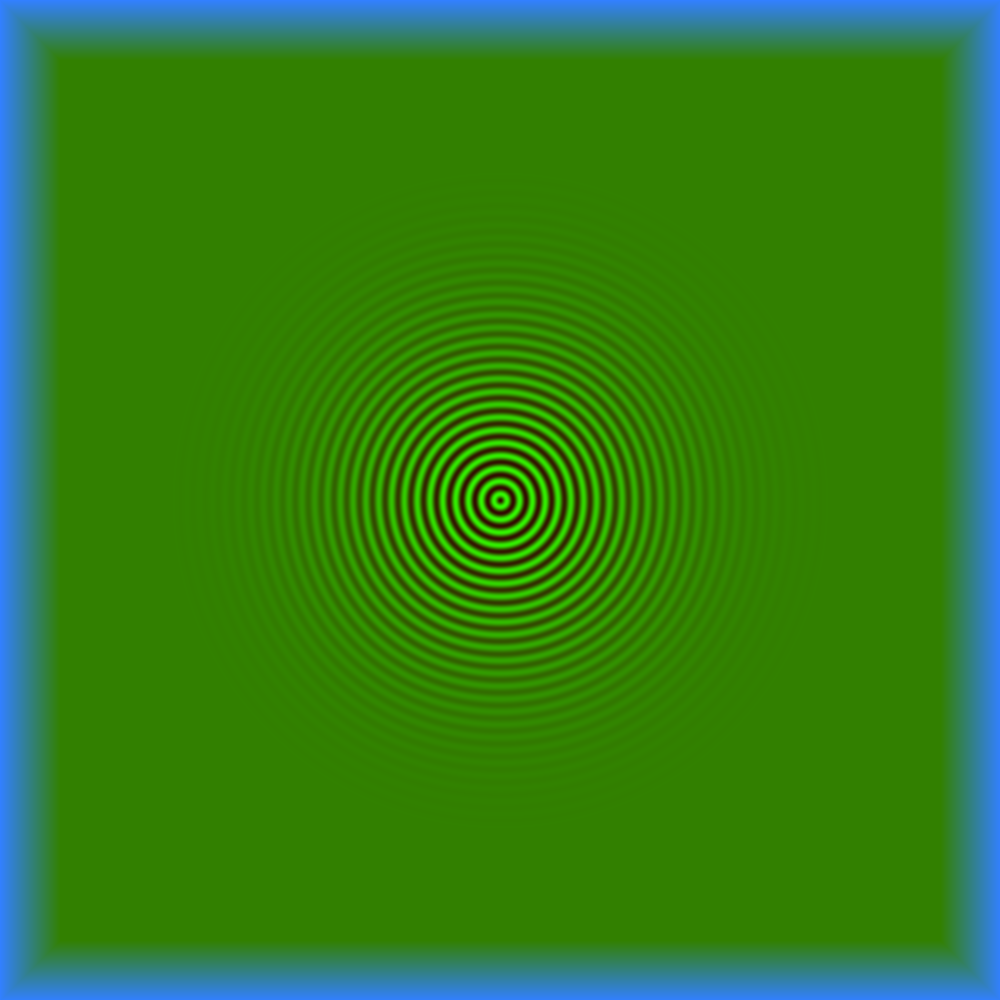
\includegraphics{papers/particles/figures/wavesim/particle_initial_state.png}
    \caption{Asymmetrischer Feldkonfiguration, die entsteht, wenn die gefangenen Energiemenge ausreichend abgenommen hat.\ \mytodo{Bild anpassen}}\label{particles:fig:partikel:abnehmen:asymmetrisch}
\end{figure}
In einer nächsten Phase wird die Symmetrie der Feldanordnung gebrochen, 
vermutlich da die gespeicherte Energie und somit die Grösse der Anordnung zu klein wird.
Aufgrund des Längenelements der ortsdiskreten Simulation sind wohl ab einer gewissen Grösse keine symmetrischen Anordnungen mehr möglich, welche stabil sind.
Die konzentrierte Energie bleibt jedoch einen weiteren Moment bestehen, 
wie die Abbildung~\ref{particles:fig:partikel:abnehmen:asymmetrisch} zeigt.

\begin{figure}
    \begin{center}
        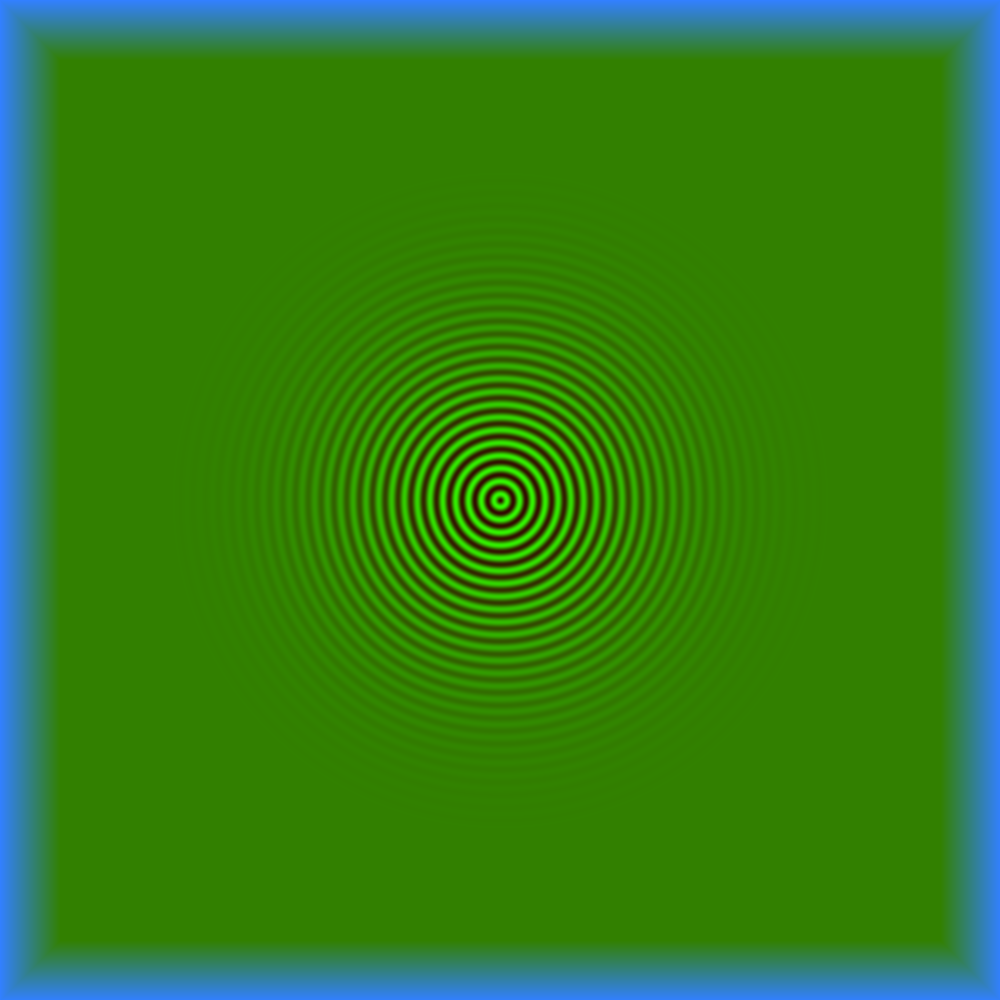
\includegraphics[width=0.5\textwidth]{papers/particles/figures/wavesim/particle_initial_state.png}
        \caption{Schlussendlicher Zerfall der Energieansammlung.\ \mytodo{Bild anpassen}}\label{particles:fig:partikel:abnehmen:zerfall}
    \end{center}
\end{figure}
In der letzten Phase wird die Energie zu klein, um die Anordnung aufrechtzuerhalten. 
Sie verfällt schliesslich in eine konzentrische, sehr hochfrequente Welle. 
Dessen Wellenlänge ist die in der Simulation kleinstmögliche, sprich zweimal das Längenelement.
Der Zerfall der Feldanordnung ist in Abbildung~\ref{particles:fig:partikel:abnehmen:zerfall} gezeigt.

% Doch was geschieht hier genau? 
% \mynote{Analogie zu Schwingkreis herstellen.}
% \mynote{Hat das Medium eine Eigenfrequenz? Falls ja, ist diese ausschlaggebend, ob sich die Energie fängt?}
% \mynote{Kann man dies als \emph{Soliton} bezeichnen?}

 % TODO: Wie funktioniert die Simulation?
% TODO Teil 3:
% - Wellengleichung
% - Diskretisierung
% - Verbindung zur Simulation (?)
%
% teil3.tex -- Beispiel-File für Teil 3
%
% (c) 2020 Prof Dr Andreas Müller, Hochschule Rapperswil
%
% !TEX root = ../../buch.tex
% !TEX encoding = UTF-8
%
\section{Fazit\label{particles:section:fazit}}
\kopfrechts{Fazit}
Sed ut perspiciatis unde omnis iste natus error sit voluptatem
accusantium doloremque laudantium, totam rem aperiam, eaque ipsa
quae ab illo inventore veritatis et quasi architecto beatae vitae
dicta sunt explicabo. Nemo enim ipsam voluptatem quia voluptas sit
aspernatur aut odit aut fugit, sed quia consequuntur magni dolores
eos qui ratione voluptatem sequi nesciunt. Neque porro quisquam
est, qui dolorem ipsum quia dolor sit amet, consectetur, adipisci
velit, sed quia non numquam eius modi tempora incidunt ut labore
et dolore magnam aliquam quaerat voluptatem. Ut enim ad minima
veniam, quis nostrum exercitationem ullam corporis suscipit laboriosam,
nisi ut aliquid ex ea commodi consequatur? Quis autem vel eum iure
reprehenderit qui in ea voluptate velit esse quam nihil molestiae
consequatur, vel illum qui dolorem eum fugiat quo voluptas nulla
pariatur?

\subsection{De finibus bonorum et malorum
\label{particles:subsection:malorum}}
At vero eos et accusamus et iusto odio dignissimos ducimus qui
blanditiis praesentium voluptatum deleniti atque corrupti quos
dolores et quas molestias excepturi sint occaecati cupiditate non
provident, similique sunt in culpa qui officia deserunt mollitia
animi, id est laborum et dolorum fuga. Et harum quidem rerum facilis
est et expedita distinctio. Nam libero tempore, cum soluta nobis
est eligendi optio cumque nihil impedit quo minus id quod maxime
placeat facere possimus, omnis voluptas assumenda est, omnis dolor
repellendus. Temporibus autem quibusdam et aut officiis debitis aut
rerum necessitatibus saepe eveniet ut et voluptates repudiandae
sint et molestiae non recusandae. Itaque earum rerum hic tenetur a
sapiente delectus, ut aut reiciendis voluptatibus maiores alias
consequatur aut perferendis doloribus asperiores repellat.


 % TODO: Fazit: Was könnten wir hier beobachtet haben?

% save current state of biburlnumpenalty in temp varialbe, in case it has already been overwritten somewhere
\newcounter{oldbiburlnumpenalty}
\setcounter{oldbiburlnumpenalty}{\value{biburlnumpenalty}}

% change biburlnumpenalty, allowing linebreaks within urls in bibliography
\setcounter{biburlnumpenalty}{7000}
\printbibliography[heading=subbibliography]

% reset biburlnumpenalty to its original state
\setcounter{biburlnumpenalty}{\value{oldbiburlnumpenalty}}
\end{refsection}
